\documentclass[11pt,aspectratio=169]{beamer}
\usepackage{imaxbeamer}

\title[F23 -- Endelig volum i 1D]{Forelesning 23\\ Endelig volum-metoden: kontrollvolum, flukser og 1D diffusjon}
\subtitle{Kompendium §3.4 og første eksempel i §3.5}
\author{IMAx3012 / IMAA3012 -- Matematikk 3B}
\date{}

\tikzset{
  node1d/.style={circle, fill=black, inner sep=0pt, minimum size=1.8mm},
  randpkt/.style={rectangle, draw=red!70!black, fill=red!30, inner sep=0pt, minimum size=2.4mm},
}

\begin{document}

\begin{frame}
\titlepage
\end{frame}

\begin{frame}{I dag}
\begin{remb}{Hvor er vi?}
F20--F22: \emph{endelige differanser} -- vi tilnærmet de \emph{deriverte} i punkter. Nå: \emph{endelig volum-metoden} (EVM) -- vi skriver opp \emph{bevaringsloven} for små celler.
\end{remb}
\begin{enumerate}
\item Hvorfor endelig volum? Transportligningen -- én ligning for mange fysiske lover.
\item Fra bevaringslov på integralform til PDE, og tilbake: divergenssetningen.
\item 1D: gitter, notasjon og diskretisering $\Rightarrow$ $a_P\phi_P = a_W\phi_W + a_E\phi_E + S^u$.
\item Randbetingelser: den halve randcellen.
\item Eksempel: varmeledning i en stav (kompendiet, §3.5).
\item EVM og endelige differanser -- likt og ulikt.
\end{enumerate}
\end{frame}

\section{Idéen}

\begin{frame}{Hvorfor en ny metode?}
\begin{columns}[T]
\begin{column}{0.49\textwidth}
\textbf{Endelige differanser}
\begin{itemize}
\item Utgangspunkt: differensialligningen.
\item Tilnærm $u'$, $u''$ i \emph{punkter}.
\item Enkelt og raskt -- på pene, rektangulære gitre.
\end{itemize}
\end{column}
\begin{column}{0.49\textwidth}
\textbf{Endelig volum}
\begin{itemize}\small
\item Utgangspunkt: \emph{bevaringsloven} (F19), på integralform.
\item \textbf{Bevaring innebygd:} fluks ut av én celle = fluks inn i neste.
\item \textbf{Vilkårlig geometri:} celler av alle former.
\item \textbf{Hopp:} materialgrenser, sjokk -- integralformen gir mening uten deriverte.
\item \textbf{Fysisk tolkning:} flukser og kilder.
\end{itemize}
\end{column}
\end{columns}
\vspace{0.3em}
\begin{remb}{I praksis}
\small EVM er standardmetoden i strømningsprogramvare (CFD: OpenFOAM, Ansys Fluent). Prisen: litt mer bokføring.
\end{remb}
\end{frame}

\begin{frame}{Utledning: bevaring for et fast kontrollvolum}
$\phi$ = størrelse \emph{per masseenhet} ($\phi=1$: masse, $\phi=u$: bevegelsesmengde, $\phi=i$: indre energi), $\rho\phi$ = per volum. Fast kontrollvolum $KV$, overflate $\partial KV$, utadrettet normal $\hat{\vect n}$, strømning $\vect u$. Tre måter $\phi$ kan endre seg på:
\begin{itemize}
\item \textbf{Konveksjon:} føres med strømmen, fluks $\rho\phi\,\vect u$.
\item \textbf{Diffusjon:} sprer seg fra høyt til lavt, fluks $-\Gamma\nabla\phi$ (Fourier, Fick).
\item \textbf{Kilder:} produseres med rate $S_\phi$ per volum.
\end{itemize}
\begin{oppsumb}{Bevaringsloven på integralform}
\small
\[
\underbrace{\frac{d}{dt}\iiint_{KV}\!\rho\phi\,dV}_{\text{økning i } KV}
+ \underbrace{\iint_{\partial KV}\!\hat{\vect n}\cdot(\rho\phi\,\vect u)\,dS}_{\text{netto ut ved konveksjon}}
= \underbrace{\iint_{\partial KV}\!\hat{\vect n}\cdot(\Gamma\nabla\phi)\,dS}_{\text{netto inn ved diffusjon}}
+ \underbrace{\iiint_{KV}\!S_\phi\,dV}_{\text{produksjon}}
\]
\end{oppsumb}
\end{frame}

\begin{frame}{Fra integralform til transportligningen}
Divergenssetningen på de to flateintegralene ($KV$ ligger fast, så $\frac{d}{dt}$ kan flyttes inn):
\[
\iiint_{KV}\left[\frac{\partial(\rho\phi)}{\partial t} + \nabla\cdot(\rho\phi\,\vect u) - \nabla\cdot(\Gamma\nabla\phi) - S_\phi\right]dV = 0
\quad\text{for \emph{alle} } KV
\]
$\Rightarrow$ integranden er null:
\begin{oppsumb}{Transportligningen}
\[
\frac{\partial(\rho\phi)}{\partial t} + \nabla\cdot(\rho\phi\,\vect u) = \nabla\cdot(\Gamma\nabla\phi) + S_\phi
\]
\end{oppsumb}
\begin{remb}{Materialderivert (Euler vs.\ Lagrange)}
Med massebevaring blir venstresiden $\rho\dfrac{D\phi}{Dt}$, der $\dfrac{D\phi}{Dt}=\dfrac{\partial\phi}{\partial t}+\vect u\cdot\nabla\phi$ er endringen for en \emph{væskepartikkel}. EVM bruker den konservative formen.
\end{remb}
\end{frame}

\begin{frame}{Én ligning -- mange fysiske lover}
Velg $\phi$, $\Gamma$ og $S_\phi$:
\begin{center}
\small
\renewcommand{\arraystretch}{1.35}
\begin{tabular}{cccl}
\toprule
$\phi$ & $\Gamma$ & $S_\phi$ & Ligning \\
\midrule
$1$ & $0$ & $0$ & Massebevaring (kontinuitet) \\
$u$ ($v$, $w$) & $\mu$ & $-\frac{\partial p}{\partial x} + S_{Mx}$ & Navier--Stokes ($S$ = krefter) \\
$i$ & $k/c_v$ & $-p\,\nabla\!\cdot\vect u + \Phi + S_i$ & Energi ($S$ = arbeid + varme) \\
$T$ ($\vect u=\vect 0$) & $\kappa/c$ & $S/c$ & Varmeligningen fra F19 \\
$Y$ (massefraksjon) & $\rho D$ & reaksjoner & Spredning av et stoff (forurensning) \\
\bottomrule
\end{tabular}
\end{center}
\begin{itemize}
\item Navier--Stokes = Newtons 2.\ lov for væsken; energiligningen = termodynamikkens 1.\ lov.
\item Systemet lukkes med tilstandsligninger, f.eks.\ $p=\rho RT$ og $i=c_vT$ (ideell gass).
\item \emph{Én} numerisk metode for transportligningen dekker alt dette.
\end{itemize}
\end{frame}

\begin{frame}{EVM: integrer over hver celle}
EVM går \emph{den motsatte veien}: del området i celler, integrer transportligningen over hver celle, og bruk divergenssetningen:
\begin{oppsumb}{Utgangspunktet for EVM}
\[
\frac{\partial}{\partial t}\iiint_{KV}\!\rho\phi\,dV + \iint_{\partial KV}\!\hat{\vect n}\cdot(\rho\phi\,\vect u)\,dS
= \iint_{\partial KV}\!\hat{\vect n}\cdot(\Gamma\nabla\phi)\,dS + \iiint_{KV}\!S_\phi\,dV
\]
\end{oppsumb}
-- bevaringsloven igjen, nå for \emph{hver celle}. Metoden: tilnærm fluksene over celleflatene og kildene i cellene.
\begin{remb}{Hele metoden i én setning}
Del området i celler. Integrer over hver celle. Tilnærm fluksene over celleflatene. Løs ligningssystemet.
\end{remb}
\end{frame}

\begin{frame}{Det enkleste tilfellet: ren, stasjonær diffusjon}
Ingen tidsavhengighet og ingen strømning ($\vect u=\vect 0$):
\begin{oppsumb}{Stasjonær diffusjon}
\[
\nabla\cdot(\Gamma\,\nabla\phi) + S = 0
\qquad\Longrightarrow\qquad
\iint_{\partial KV}\hat{\vect n}\cdot(\Gamma\nabla\phi)\,dS + \iiint_{KV} S\,dV = 0 .
\]
\end{oppsumb}
\begin{itemize}
\item Diffusiv fluks \emph{inn} gjennom overflaten + produksjon inne i KV $=0$.
\item F23--F26: ren diffusjon i 1D (i dag og F24), 2D (F25) og med tid (F26).
\item Konveksjonsleddet (og dermed Navier--Stokes) behandles med de samme ideene, men er utenfor pensum.
\end{itemize}
\end{frame}

\section{EVM i 1D}

\begin{frame}{1D: celler, noder og flater}
Stasjonær 1D-diffusjon: $\dfrac{d}{dx}\left(\Gamma\dfrac{d\phi}{dx}\right) + S = 0$ på et intervall mellom randene $V$ og $H$.
\begin{center}
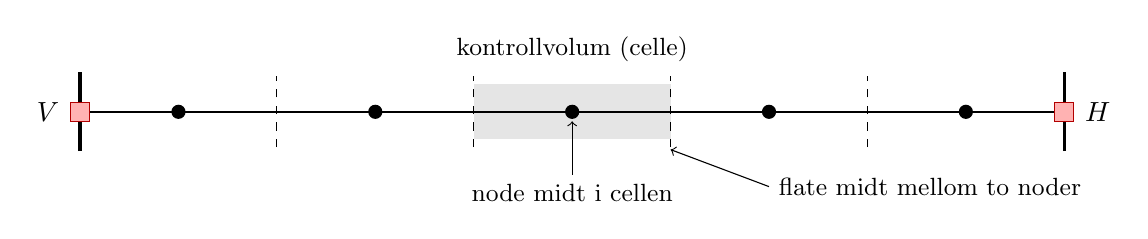
\begin{tikzpicture}[x=1.25cm]
\fill[gray!20] (4,-0.35) rectangle (6,0.35);
\draw[thick] (0,0) -- (10,0);
\foreach \x in {0,10} \draw[very thick] (\x,-0.5) -- (\x,0.5);
\foreach \x in {2,4,6,8} \draw[dashed] (\x,-0.45) -- (\x,0.45);
\foreach \x in {1,3,5,7,9} \node[node1d] at (\x,0) {};
\node[randpkt] at (0,0) {}; \node[randpkt] at (10,0) {};
\node[left=4pt] at (0,0) {$V$}; \node[right=4pt] at (10,0) {$H$};
\node[above=6pt, font=\small] at (5,0.3) {kontrollvolum (celle)};
\draw[<-] (5,-0.12) -- (5,-0.8) node[below, font=\small] {node midt i cellen};
\draw[<-] (6,-0.48) -- (7,-0.95) node[right, font=\small] {flate midt mellom to noder};
\end{tikzpicture}
\end{center}
\begin{enumerate}
\item Plasser noder mellom $V$ og $H$.
\item Legg cellegrensene (\emph{flatene}) midt mellom nabonodene. Hver node er omgitt av sin celle.
\item Randene $V$ og $H$ faller sammen med celleflater.
\end{enumerate}
\end{frame}

\begin{frame}{Notasjon}
\begin{center}
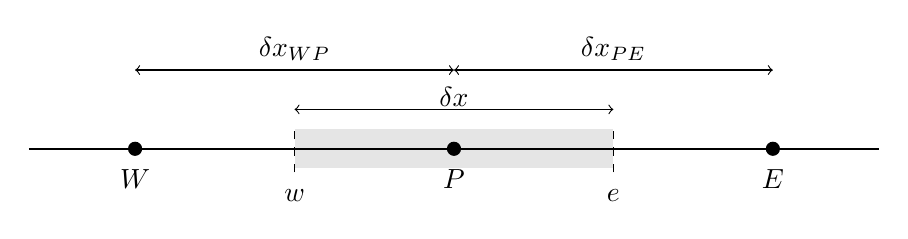
\begin{tikzpicture}[x=1.35cm]
\fill[gray!20] (2.5,-0.25) rectangle (5.5,0.25);
\draw[thick] (0,0) -- (8,0);
\draw[dashed] (2.5,-0.3) -- (2.5,0.3); \draw[dashed] (5.5,-0.3) -- (5.5,0.3);
\node[node1d] (W) at (1,0) {}; \node[node1d] (P) at (4,0) {}; \node[node1d] (E) at (7,0) {};
\node[below=4pt] at (1,0) {$W$}; \node[below=4pt] at (4,0) {$P$}; \node[below=4pt] at (7,0) {$E$};
\node[below=4pt] at (2.5,-0.25) {$w$}; \node[below=4pt] at (5.5,-0.25) {$e$};
\draw[<->] (1,1.0) -- (4,1.0) node[midway, above] {$\delta x_{WP}$};
\draw[<->] (4,1.0) -- (7,1.0) node[midway, above] {$\delta x_{PE}$};
\draw[<->] (2.5,0.5) -- (5.5,0.5) node[midway, above, fill=white, inner sep=1pt] {$\delta x$};
\end{tikzpicture}
\end{center}
\begin{itemize}
\item Store bokstaver = \textbf{noder}: $P$ (den vi ser på), $W$ (vest), $E$ (øst).
\item Små bokstaver = \textbf{flater}: $w$ og $e$.
\item Senketegn = verdi i punktet: $\phi_P$, $\Gamma_e$, \ldots
\item Uniformt gitter: $\delta x_{WP}=\delta x_{PE}=\delta x$ (cellebredden).
\end{itemize}
\end{frame}

\begin{frame}{Steg 2: integrer over cellen rundt $P$}
\begin{center}
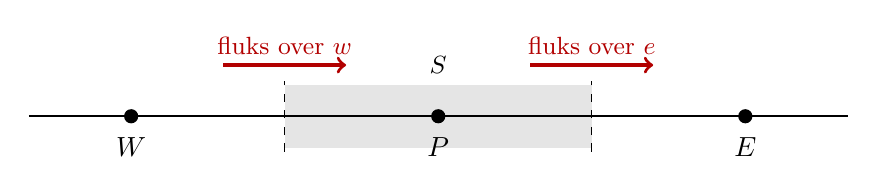
\begin{tikzpicture}[x=1.3cm]
\fill[gray!20] (2.5,-0.4) rectangle (5.5,0.4);
\draw[thick] (0,0) -- (8,0);
\draw[dashed] (2.5,-0.45) -- (2.5,0.45); \draw[dashed] (5.5,-0.45) -- (5.5,0.45);
\node[node1d] at (1,0) {}; \node[node1d] at (4,0) {}; \node[node1d] at (7,0) {};
\node[below=4pt] at (1,0) {$W$}; \node[below=4pt] at (4,0) {$P$}; \node[below=4pt] at (7,0) {$E$};
\draw[->, very thick, red!70!black] (1.9,0.65) -- (3.1,0.65) node[above, midway, font=\small] {fluks over $w$};
\draw[->, very thick, red!70!black] (4.9,0.65) -- (6.1,0.65) node[above, midway, font=\small] {fluks over $e$};
\node[font=\small] at (4,0.65) {$S$};
\end{tikzpicture}
\end{center}
Integralet av $\frac{d}{dx}(\cdot)$ over cellen er bare differansen mellom flatene:
\[
\iiint_{KV}\frac{d}{dx}\!\left(\Gamma\frac{d\phi}{dx}\right)dV + \iiint_{KV} S\,dV
= \left(\Gamma A\frac{d\phi}{dx}\right)_e - \left(\Gamma A\frac{d\phi}{dx}\right)_w + \overline S\,\Delta V = 0 .
\]
\begin{remb}{Problemet}
Vi trenger $\Gamma$ og $\dfrac{d\phi}{dx}$ på \emph{flatene} $e$ og $w$ -- men vi kjenner (og leter etter) $\phi$ bare i \emph{nodene}.
\end{remb}
\end{frame}

\begin{frame}{Tilnærming av fluksene: rett linje mellom nodene}
\begin{columns}[c]
\begin{column}{0.42\textwidth}
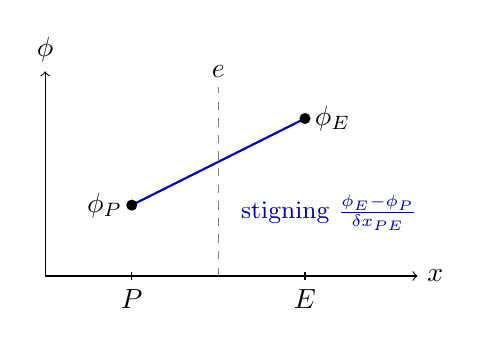
\begin{tikzpicture}[x=1.1cm, y=1cm]
\draw[->] (0,0) -- (4.3,0) node[right] {$x$};
\draw[->] (0,0) -- (0,2.6) node[above] {$\phi$};
\draw[dashed, gray] (2,0) -- (2,2.4) node[above, black] {$e$};
\draw[thick, blue!70!black] (1,0.9) -- (3,2.0);
\fill (1,0.9) circle (2pt) node[left] {$\phi_P$};
\fill (3,2.0) circle (2pt) node[right] {$\phi_E$};
\draw (1,0.05) -- (1,-0.05) node[below] {$P$};
\draw (3,0.05) -- (3,-0.05) node[below] {$E$};
\node[font=\small, blue!70!black, anchor=north west] at (2.15,1.15) {stigning $\frac{\phi_E-\phi_P}{\delta x_{PE}}$};
\end{tikzpicture}
\end{column}
\begin{column}{0.56\textwidth}
\begin{oppsumb}{Sentral tilnærming}
\small
\[
\left(\Gamma A\frac{d\phi}{dx}\right)_e \approx \Gamma_e A_e\frac{\phi_E-\phi_P}{\delta x_{PE}}
\]
\[
\left(\Gamma A\frac{d\phi}{dx}\right)_w \approx \Gamma_w A_w\frac{\phi_P-\phi_W}{\delta x_{WP}}
\]
Uniformt gitter: $\Gamma_e=\frac{\Gamma_P+\Gamma_E}{2}$, $\Gamma_w=\frac{\Gamma_W+\Gamma_P}{2}$.
\end{oppsumb}
\end{column}
\end{columns}
\medskip
Kilden skrives på lineær form: $\overline S\,\Delta V = S^u + S_P\phi_P$ \;(mer om dette i F24).
\end{frame}

\begin{frame}{Den diskrete ligningen}
Setter vi inn tilnærmingene:
\[
\Gamma_eA_e\frac{\phi_E-\phi_P}{\delta x_{PE}} - \Gamma_wA_w\frac{\phi_P-\phi_W}{\delta x_{WP}} + S^u + S_P\phi_P = 0 .
\]
Samle $\phi_P$ på venstre side:
\begin{oppsumb}{EVM-ligningen for celle $P$}
\[
a_P\,\phi_P = a_W\,\phi_W + a_E\,\phi_E + S^u,
\quad
a_W = \frac{\Gamma_wA_w}{\delta x_{WP}},\ \ a_E = \frac{\Gamma_eA_e}{\delta x_{PE}},\ \ a_P = a_W + a_E - S_P .
\]
\end{oppsumb}
\begin{itemize}
\item $a_W$, $a_E$ er \emph{ledningsevner}: hvor lett $\phi$ strømmer mellom $P$ og naboen.
\item Én slik ligning per celle $\Rightarrow$ et \emph{tridiagonalt} ligningssystem.
\item $S_P\le 0$ gjør $a_P$ større, og systemet «snillere».
\end{itemize}
\end{frame}

\begin{frame}{Bevaring er innebygd}
\begin{center}
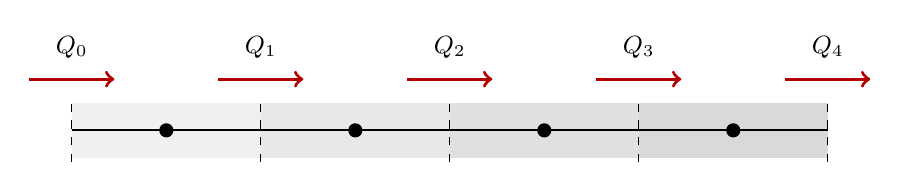
\begin{tikzpicture}[x=1.2cm]
\foreach \i in {0,...,3} \fill[gray!\the\numexpr 12+6*\i\relax] (2*\i,-0.35) rectangle (2*\i+2,0.35);
\draw[thick] (0,0) -- (8,0);
\foreach \x in {0,2,4,6,8} \draw[dashed] (\x,-0.4) -- (\x,0.4);
\foreach \x in {1,3,5,7} \node[node1d] at (\x,0) {};
\foreach \x in {0,2,4,6,8} \draw[->, very thick, red!70!black] (\x-0.45,0.65) -- (\x+0.45,0.65);
\foreach \x/\l in {0/Q_0,2/Q_1,4/Q_2,6/Q_3,8/Q_4} \node[above=1pt, font=\small] at (\x,0.75) {$\l$};
\end{tikzpicture}
\end{center}
\begin{itemize}
\item Fluksen $Q_i$ over en flate regnes ut med \emph{samme} formel fra begge sider: det som går ut av én celle, går \emph{nøyaktig} inn i neste.
\item Summer vi ligningene for alle cellene, kansellerer alle de indre fluksene:
\[
Q_{\text{ut}} - Q_{\text{inn}} = \sum_{\text{celler}} \overline S\,\Delta V .
\]
\end{itemize}
\begin{remb}{Konservativ metode}
Den diskrete løsningen oppfyller bevaringsloven \emph{eksakt} -- for hele området og for hver celle -- uansett hvor grovt gitteret er.
\end{remb}
\end{frame}

\begin{frame}{Steg 3: randbetingelser -- den halve randcellen}
\begin{center}
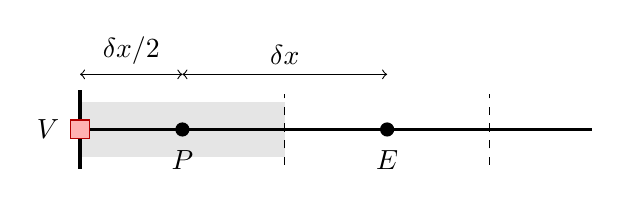
\begin{tikzpicture}[x=1.3cm]
\fill[gray!20] (0,-0.35) rectangle (2,0.35);
\draw[thick] (0,0) -- (5,0);
\draw[very thick] (0,-0.5) -- (0,0.5); \draw[dashed] (2,-0.45) -- (2,0.45); \draw[dashed] (4,-0.45) -- (4,0.45);
\node[randpkt] at (0,0) {}; \node[left=4pt] at (0,0) {$V$};
\node[node1d] at (1,0) {}; \node[below=4pt] at (1,0) {$P$};
\node[node1d] at (3,0) {}; \node[below=4pt] at (3,0) {$E$};
\draw[<->] (0,0.7) -- (1,0.7) node[midway, above] {$\delta x/2$};
\draw[<->] (1,0.7) -- (3,0.7) node[midway, above] {$\delta x$};
\end{tikzpicture}
\end{center}
Randen $V$ \emph{er} vestflaten. Fluksen dit tilnærmes lineært mellom $T_V$ og $P$ -- over en \emph{halv} celle:
\[
\Gamma A\frac{\phi_E-\phi_P}{\delta x} - \Gamma A\frac{\phi_P-\phi_V}{\delta x/2} = 0 .
\]
\begin{oppsumb}{Randcelle med kjent verdi $\phi_V$: «kutt koblingen»}
\[
a_W = 0, \qquad S^u = \frac{2\Gamma A}{\delta x}\,\phi_V, \qquad S_P = -\frac{2\Gamma A}{\delta x}
\]
Randverdien bakes inn som et kildeledd -- formen $a_P\phi_P = a_W\phi_W + a_E\phi_E + S^u$ er uendret.
\end{oppsumb}
\end{frame}

\begin{frame}{Generelt: konstant $\Gamma A$ og fast $\delta x$ -- en tridiagonal matrise}
\small
Med $N$ celler, kjent $\phi_V$ og $\phi_H$ og ingen kilde. Kall $c = \dfrac{\Gamma A}{\delta x}$:
\begin{columns}[c]
\begin{column}{0.44\textwidth}
\centering\footnotesize
\setlength{\tabcolsep}{3.5pt}
\begin{tabular}{cccccc}
\toprule
Node & $a_W$ & $a_E$ & $S^u$ & $S_P$ & $a_P$ \\
\midrule
$1$ & $0$ & $c$ & $2c\,\phi_V$ & $-2c$ & $3c$ \\
$2,\ldots,N-1$ & $c$ & $c$ & $0$ & $0$ & $2c$ \\
$N$ & $c$ & $0$ & $2c\,\phi_H$ & $-2c$ & $3c$ \\
\bottomrule
\end{tabular}
\end{column}
\begin{column}{0.54\textwidth}
\footnotesize
\setlength{\arraycolsep}{2.5pt}
\[
c\begin{bmatrix}
\textcolor{red!70!black}{3} & -1 & & & \\
-1 & 2 & -1 & & \\
 & \ddots & \ddots & \ddots & \\
 & & -1 & 2 & -1 \\
 & & & -1 & \textcolor{red!70!black}{3}
\end{bmatrix}
\begin{bmatrix} \phi_1\\ \phi_2\\ \vdots\\ \phi_{N-1}\\ \phi_N \end{bmatrix}
=
c\begin{bmatrix} \textcolor{red!70!black}{2}\phi_V\\ 0\\ \vdots\\ 0\\ \textcolor{red!70!black}{2}\phi_H \end{bmatrix}
\]
\end{column}
\end{columns}
\vspace{0.3em}
\begin{itemize}
\item \textbf{Tridiagonal:} hver celle kobler bare til sine to naboer. Indre rader: $-1,\ 2,\ -1$ -- som sentraldifferansen i F20.
\end{itemize}
\begin{remb}{Hvorfor faktoren $2$ (og $3$) på randene?}
Randen ligger bare $\delta x/2$ fra den ytterste noden, så ledningsevnen dit er $\frac{\Gamma A}{\delta x/2} = 2c$. Den gir $S^u = 2c\,\phi_V$ og $S_P=-2c$, og diagonalen $a_P = a_E - S_P = c + 2c = 3c$.\\
I koden: \texttt{dx[0]} $=\delta x/2$, så \texttt{kA/dx[0]} $=2c$.
\end{remb}
\end{frame}

\section{Eksempel}

\begin{frame}{Eksempel: varmeledning i en stav uten kilde}
\begin{center}
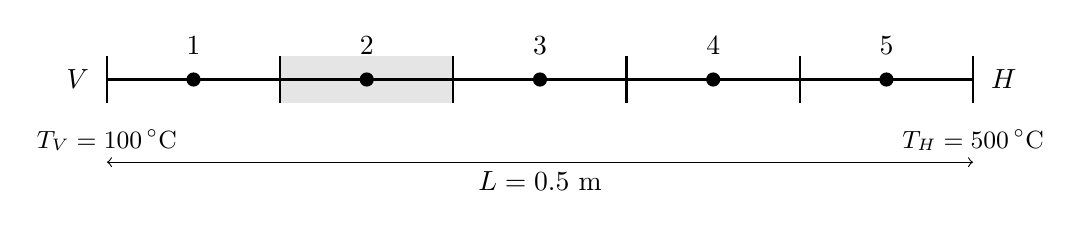
\begin{tikzpicture}[x=1.1cm]
\fill[gray!20] (2,-0.3) rectangle (4,0.3);
\draw[thick] (0,0) -- (10,0);
\foreach \x in {0,2,4,6,8,10} \draw[thick] (\x,0.3) -- (\x,-0.3);
\foreach \x/\n in {1/1,3/2,5/3,7/4,9/5} { \node[node1d] at (\x,0) {}; \node[above=4pt] at (\x,0.05) {$\n$}; }
\node[left=3pt] at (0,0) {$V$}; \node[right=3pt] at (10,0) {$H$};
\node[below=6pt, font=\small] at (0,-0.3) {$T_V=100\,^\circ$C};
\node[below=6pt, font=\small] at (10,-0.3) {$T_H=500\,^\circ$C};
\draw[<->] (0,-1.05) -- (10,-1.05) node[midway, below] {$L=0.5$ m};
\end{tikzpicture}
\end{center}
\[
\frac{d}{dx}\left(\kappa\frac{dT}{dx}\right)=0, \qquad \kappa = 1000~\tfrac{\text{W}}{\text{m\,K}}, \quad A = 10\cdot10^{-3}~\text{m}^2 .
\]
Fem celler: $\delta x = 0.1$ m, noder i $x = 0.05, 0.15, \ldots, 0.45$, og
\[
\frac{\kappa A}{\delta x} = \frac{1000\cdot 0.01}{0.1} = 100 .
\]
\end{frame}

\begin{frame}{Koeffisientene og ligningssystemet}
\begin{columns}[c]
\begin{column}{0.44\textwidth}
\centering\footnotesize
\begin{tabular}{cccccc}
\toprule
Node & $a_W$ & $a_E$ & $S^u$ & $S_P$ & $a_P$ \\
\midrule
1 & 0 & 100 & $200T_V$ & $-200$ & 300 \\
2 & 100 & 100 & 0 & 0 & 200 \\
3 & 100 & 100 & 0 & 0 & 200 \\
4 & 100 & 100 & 0 & 0 & 200 \\
5 & 100 & 0 & $200T_H$ & $-200$ & 300 \\
\bottomrule
\end{tabular}
\end{column}
\begin{column}{0.54\textwidth}
\footnotesize
\setlength{\arraycolsep}{3pt}
\[
\begin{bmatrix}
300 & -100 & & & \\
-100 & 200 & -100 & & \\
 & -100 & 200 & -100 & \\
 & & -100 & 200 & -100 \\
 & & & -100 & 300
\end{bmatrix}
\begin{bmatrix} T_1\\T_2\\T_3\\T_4\\T_5 \end{bmatrix}
=
\begin{bmatrix} 200T_V\\0\\0\\0\\200T_H \end{bmatrix}
\]
\end{column}
\end{columns}
\vspace{0.6em}
\begin{itemize}
\item Diagonal: $a_P$. Under: $-a_W$. Over: $-a_E$. Høyreside: $S^u$.
\item Tridiagonal -- hver celle kobler bare til sine to naboer.
\end{itemize}
\end{frame}

\begin{frame}{Løsningen}
\begin{columns}[c]
\begin{column}{0.55\textwidth}
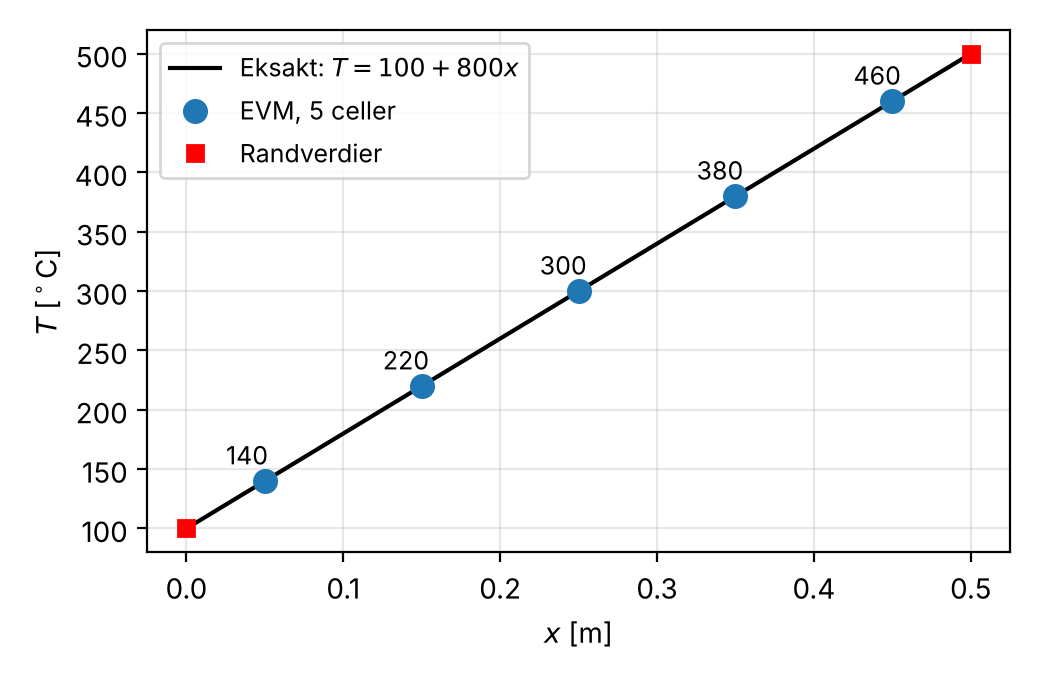
\includegraphics[width=\textwidth]{assets/stav_losning.png}
\end{column}
\begin{column}{0.43\textwidth}
\[
T_1,\ldots,T_5 = 140,\ 220,\ 300,\ 380,\ 460
\]
Eksakt: $T(x)=100+800x$ -- \emph{samme} verdier i nodene.
\begin{remb}{Hvorfor eksakt?}
Vi tilnærmet fluksene med \emph{rette linjer} mellom nodene. Er $T$ selv en rett linje, er tilnærmingen eksakt.
\end{remb}
\end{column}
\end{columns}
\end{frame}

\begin{frame}[fragile]{I koden: som i øvingene}
\begin{columns}[T]
\begin{column}{0.56\textwidth}
\begin{lstb}[Python-kode]
\begin{lstlisting}
x = np.array([0, 0.05, 0.15, 0.25, 0.35, 0.45, 0.5])
m = len(x) - 2         # antall ukjente
kA = 10
a, b = 100, 500        # T_V og T_H
dx = x[1:] - x[:-1]

L = kA*(-np.diag((1/dx)[1:-1], 1)
        - np.diag(1/dx[1:-1], -1)
        + np.diag(1/dx[1:], 0)
        + np.diag(1/dx[:-1], 0))
F = np.zeros((m))
F[0]  = kA*1/dx[0]*a
F[-1] = kA*1/dx[-1]*b
u = la.solve(L, F)
\end{lstlisting}
\end{lstb}
\end{column}
\begin{column}{0.42\textwidth}
\small
\begin{itemize}
\item \texttt{x}: \emph{alle} punkter, randpunktene først og sist. Nodene er \texttt{x[1:-1]}.
\item \texttt{dx}: avstand til nabopunktet. Ytterst: \texttt{dx[0]} $=\delta x/2$.
\item Randpunktet er en kjent nabo: $\frac{kA}{\delta x/2} = \frac{2kA}{\delta x}$ -- akkurat kompendiets $S^u$ og $S_P$.
\item Punktene trenger ikke ligge jevnt -- formlene er de samme.
\end{itemize}
\end{column}
\end{columns}
\end{frame}

\begin{frame}{Sjekk: like stor fluks gjennom hver flate}
Fluksen $Q=-\kappa A\,\dfrac{dT}{dx}$, regnet ut på hver flate (randflatene med $\delta x/2$):
\begin{center}
\begin{tabular}{lcccccc}
\toprule
Flate ($x$ i m) & 0.0 & 0.1 & 0.2 & 0.3 & 0.4 & 0.5 \\
\midrule
$Q$ (W) & $-8000$ & $-8000$ & $-8000$ & $-8000$ & $-8000$ & $-8000$ \\
\bottomrule
\end{tabular}
\end{center}
\begin{itemize}
\item Eksakt: $Q = -\kappa A\cdot 800 = -10\cdot 800 = -8000$ W (varmen går fra den varme høyre enden mot venstre).
\item Ingen varmekilde $\Rightarrow$ like mye varme gjennom hver flate. EVM får dette \emph{eksakt}, per konstruksjon.
\end{itemize}
\end{frame}

\section{EVM og endelige differanser}

\begin{frame}{EVM og endelige differanser: likt og ulikt}
Konstant $\Gamma$, $A$ og uniformt gitter: $a_W=a_E=\Gamma A/\delta x$, og for en indre celle
\[
\Gamma A\frac{\phi_E-2\phi_P+\phi_W}{\delta x} + \overline S A\,\delta x = 0
\quad\Longleftrightarrow\quad
\Gamma\frac{\phi_E-2\phi_P+\phi_W}{\delta x^2} + \overline S = 0
\]
-- \emph{akkurat} sentraldifferanseformelen fra F20!
\begin{columns}[T]
\begin{column}{0.49\textwidth}
\textbf{Likt}
\begin{itemize}
\item Indre ligninger (enkle tilfeller).
\item Tridiagonalt system, samme løsere (direkte, Jacobi, Gauss-Seidel).
\end{itemize}
\end{column}
\begin{column}{0.49\textwidth}
\textbf{Ulikt}
\begin{itemize}
\item Utgangspunkt: bevaringsloven $\Rightarrow$ eksakt diskret bevaring.
\item Noder midt i cellene $\Rightarrow$ halv randcelle.
\item Variabel $\Gamma$, ikke-uniforme gitre, vilkårlige celler.
\end{itemize}
\end{column}
\end{columns}
\end{frame}

\begin{frame}{Utblikk: en stav av to materialer \hfill {\small\color{red}\textbf{(Ikke pensum)}}}
\begin{columns}[c]
\begin{column}{0.56\textwidth}
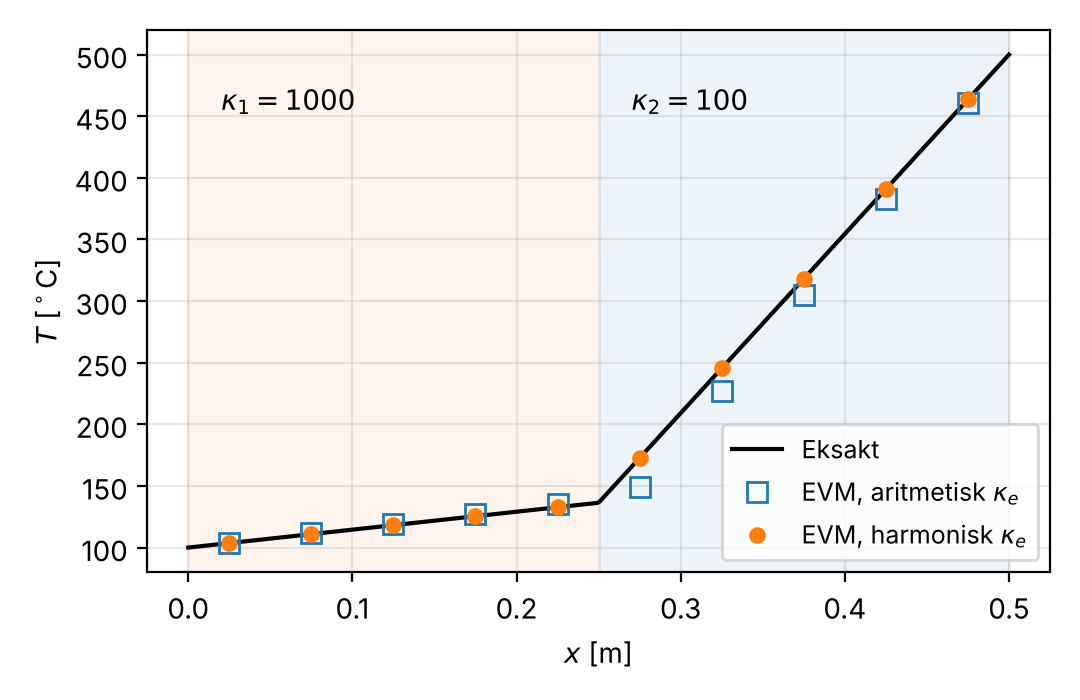
\includegraphics[width=\textwidth]{assets/to_materialer.png}
\end{column}
\begin{column}{0.42\textwidth}
\small
Venstre halvdel $\kappa_1=1000$, høyre $\kappa_2=100$; 10 celler. Grenseflaten er en celleflate.
\begin{itemize}
\item Aritmetisk $\kappa_e$: feil opptil $23\,^\circ$C.
\item \emph{Harmonisk} $\kappa_e=\dfrac{2\kappa_P\kappa_E}{\kappa_P+\kappa_E}$: eksakt!
\end{itemize}
\begin{remb}{Hvorfor?}
Varmen går gjennom to halve celler etter hverandre -- to seriekoblede «motstander». Å tenke i \emph{flukser over flater} gir svaret direkte.
\end{remb}
\end{column}
\end{columns}
\end{frame}

\begin{frame}{Oppsummering}
\begin{oppsumb}{Endelig volum-metoden, steg for steg}
\begin{enumerate}
\item \textbf{Gitter:} del området i celler; noder i midten, flater midt mellom nodene, randene på flater.
\item \textbf{Diskretiser:} integrer over hver celle (divergenssetningen) og tilnærm fluksene lineært:
\[
a_P\phi_P = a_W\phi_W + a_E\phi_E + S^u, \qquad a_P = a_W + a_E - S_P .
\]
Randceller: kutt koblingen og legg randbidraget i $S^u$, $S_P$.
\item \textbf{Løs} det (tridiagonale) ligningssystemet.
\end{enumerate}
\end{oppsumb}
\begin{itemize}
\item Metoden er \emph{konservativ}: fluksen ut av én celle er fluksen inn i neste.
\item Kode: \texttt{F23\_EVM\_1D\_Diffusjon.ipynb}.
\end{itemize}
\end{frame}

\begin{frame}{Neste gang: F24 -- kildeledd og andre randbetingelser}
\begin{nestefb}
\begin{itemize}
\item Kildeledd: $\overline S\,\Delta V = S^u + S_P\phi_P$ -- og hvorfor $S_P\le 0$.
\item Eksempler fra kompendiet: plate med varmeproduksjon, og ribbe som kjøles av luft.
\item Isolert rand og kjent fluks (Neumann).
\item Koding: vi utvider F23-løseren.
\end{itemize}
\end{nestefb}
\end{frame}

\end{document}
